\subsection{Motivation}
The consensus algorithm designed by the engineers and researchers at Atlas City rests on the principle that every node participating in the network can contribute to the ledger state update and should be rewarded accordingly. Indeed, the consensus mechanism was conceived based on the observations that:  \\

\begin{itemize}
\item In reality, not every node needs to validate every transaction for a network to be secure and a ledger fully decentralised. 
\item Collectively across a network of nodes there is significant distributed computer resources to build a trusted ledger. Network performance should as a result improve as the network scales up.
\end{itemize}

The PoW algorithm was introduced to solve the General Byzantine Problem among participants in the peer-to-peer network, allowing them to reach consensus without trusting one another~\cite{BFT}. In the PoW algorithm or any derivatives, mining nodes collect and validate all transactions broadcast to the network and form a block with these new transactions. The miners compete to solve a computationally hard problem, the solution of which is used to prove that a block is valid and can therefore be appended to the blockchain. The level of difficulty attached to the cryptographic problem solved by the miners is set by the network to ensure that blocks are produced on a regular time interval (roughly 10 minutes in the case of Bitcoin, and approximatively 17s for Ethereum). Under this scenario, one mining node is rewarded for producing the correct next block of the blockchain (which in the analogy of Catalyst corresponds to the last valid ledger state update). Although the solution to the cryptographic puzzle is hard to find, it is very easy to verify which allow for a fast and secure update of the blockchain.  \\

While this approach provides a secure way to maintain a distributed ledger, it leads to a tremendous amount of wasted computational and electrical energy with high risk of mining centralisation. In the example of Bitcoin, the early blocks were mined by individuals with modest computer resource. \\

\begin{figure}[H]
\center{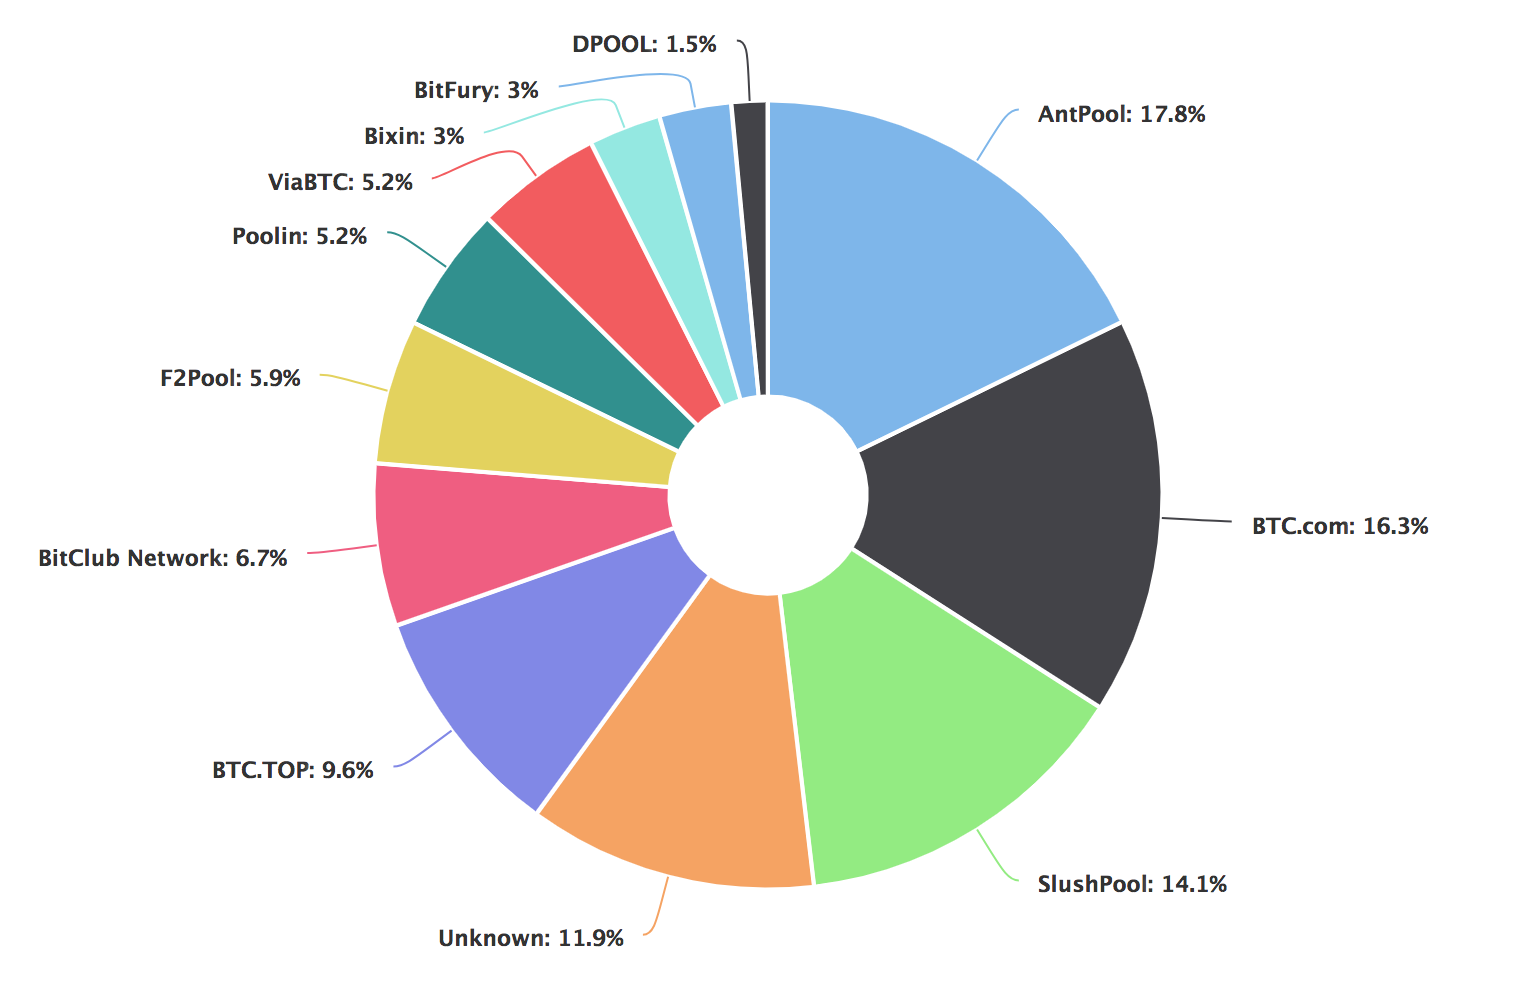
\includegraphics[width=11cm]{Figures/BTC_mining_pools_2018-10-30}}
\caption{\label{fig:pools} Distribution of the Bitcoin hashrate power over a 24h period, as the 30 of October 2018\cite{bc24}}
\end{figure}

As illustrated in Figure~\ref{fig:pools}, the situation is rather different nowadays. Few miners work independently (represented as the “unknown” 11.9\%) while the remaining join mining pools such as Slush Pool (which was the first mining pool created for Bitcoin mining) to share their computer resources and the collected rewards, usually against the payment of a fee (2\% of the mining reward with Slush Pool). Some mining pools are private pool, such as BTC.top. It also worth noting that around 80\% of the mining pools are located in China~\cite{pool_cent} where the electricity is considerably cheaper than in other parts of the world.   \\

A popular alternative to the PoW algorithm currently considered by several blockchain projects is the Proof-of-Stake algorithm (PoS). This approach addresses the footprint concerns from the former by assigning the task of producing the next valid bock to a subset of miners. The miner nodes can be selected randomly or based on criteria such as the miner’s wealth (stake). The main concern with a PoS-based consensus mechanism is the risk for centralisation of wealth and subsequently the network management, with the mining work inevitably distributed to a few wealthy nodes~\cite{PoSr}.\\

\textbf{\textit{Unity is strength}}\\
Catalyst consensus mechanism is not based on a competitive process. Instead, the nodes in the network collaborate to collectively build the correct update of the ledger state. At the end of a ledger cycle, new tokens are injected into the system and all the nodes that contributed to producing the correct ledger state update receive a share of that reward.

\subsection{Naming Convention}

Nodes who contribute to maintaining the ledger state are called producers, rather than miners. Indeed, producers do not solve a computationally hard problem, but instead validate the transactions broadcast to the network and use these to collaboratively build (produce) a ledger state update. \\

In this chapter we assume that the ledger is composed of one single shard comprising a fixed set of accounts. The implementation of sharding techniques are discussed in chapter~\ref{Sec:Sca}. We therefore consider one single pool of workers and one subset of producer nodes selected per ledger cycle. \\

A ledger cycle $C_n$ starts at time $t = t_{n,0}$ and lasts for a period of time $\Delta t_{cycle}$, therefore ending at $t = t_{n,0}+ \Delta t_{cycle}$. $P$ producers $\{P_j\}_{j\in P}$ are selected to build the ledger state update during the ledger cycle $C_n$. Each producer $P_j$ can be identified by its peers as well as the rest of the network via its unique identifier $Id_j$.\\

During $C_n$ the $P$ producers collaborate to create a ledger state update $\Delta L_{n}$ based on the set of $m_{n-1}$ transactions broadcast on the network during the previous ledger cycle $C_{n-1}$. To limit discrepancies in the set of transactions collected by the different producers and processed during $C_n$ a small time window $\Delta t_{freeze}$ is considered. The $m_{n-1}$ transactions $\{Tx_j\}_{j=1,..,m_{n-1}}$ are actually collected during the period of time [$t_{0,n-1} - \Delta t_{freeze}, t_{n,0}$] ($t_{n-1,0} = t_{n,0} - \Delta t_{cycle}$) and must have a timestamp comprised between $t_{0,n-1} - \Delta t_{freeze}$ and $t_{n,0} - \Delta t_{freeze}$.\\

Each producer compiles a ledger state update and interacts with its peers to vote on the most popular ledger state update produced by the set of producers. Each producer is thus tasked with two responsibilities: compiling a local ledger state update and voting on the correct (most popular) ledger state update. Each task entitles the producer to receive part of the reward allocated to producers for maintaining the ledger state. The amount of reward individually collected depends on the quality of work performed by a producer. During a ledger cycle $C_n$ two lists of producer identifiers are created, $\mathcal{L}_n(prod)$ and $\mathcal{L}_n(vote)$. The first one lists the identifiers of producers who correctly built the ledger state update while the second one lists the identifiers of producers who correctly voted on the correct ledger state update built by the producers included in the first list.\\


Throughout the different phases of the ledger cycle, the producers exchange quantities that are hashes, notably of ledger state updates, (using the $Blake-2b$ hashing function) to which they append their identifiers. The exchange of hashes allows for fast and efficient communication rounds amongst the peers as these are smaller pieces of data than the actual ledger state updates. \\

The ledger cycle is composed of three phases. Namely, a computation phase during which the producers locally generate a ledger state update, a voting phase during which the producers reach consensus on the correct set of changes to distribute to the rest of the network and a synchronisation phase during which the correct update including the reward to producers is distributed and the ledger state  is updated by all nodes in the network. 
